% questions.tex -- Module 5 (Advanced Mechanics) short-answer booklet, SET 2 (HSC Section II style).
% 20 new questions, 90 marks: Topic 1 Q1-6 (26 marks), Topic 2 Q7-13 (32), Topic 3 Q14-20 (32).
% Does not repeat Set 1 (src/m5_short_answer/). Same plain layout (quiz.sty).
% Marking guidelines and sample answers: answers.tex.
% Every number: checks/m5-short-answer-2/numbers.py
% Build: TEXINPUTS=.: xelatex questions.tex (twice)
\documentclass[12pt]{article}
\usepackage{quiz}
\hypersetup{pdftitle={Short Answer Questions Set 2 - Module 5 - Advanced Mechanics}}

\begin{document}
\quiztitle{Year 12 Physics}{Short Answer Questions (Set 2) - Module 5 - Advanced Mechanics}
\begin{center}
  20 questions \textperiodcentered\ 90 marks \textperiodcentered\ allow about 2 hours 40 minutes\\[2pt]
  Show all working. Use $g = \qty{9.8}{m.s^{-2}}$, $G = \qty{6.67e-11}{N.m^2.kg^{-2}}$,
  $M_\mathrm{E} = \qty{6.0e24}{kg}$, $r_\mathrm{E} = \qty{6.371e6}{m}$.
\end{center}

% =====================================================================
\firsttopictitle{Topic 1 - Projectile Motion}

% ---- Q1 (basketball shot)
\begin{saq}{4}
A basketball is released from a height of \qty{2.0}{m} above the floor with a velocity of
\qty{8.5}{m.s^{-1}} at \ang{52} above the horizontal. Ignore air resistance.
\qpartL{a}{2}{Calculate the maximum height of the ball above the floor.}{5}
\qpartL{b}{1}{Calculate the speed of the ball at its maximum height.}{2}
\qpartL{c}{1}{Explain why the acceleration of the ball is not zero at its maximum height.}{2}
\end{saq}

% ---- Q2 (derive the range equation)
\Needspace{24\baselineskip}
\begin{saq}{5}
A projectile is launched from level ground with speed $u$ at an angle $\theta$ above the horizontal,
and lands at the same height. Ignore air resistance.
\qpartL{a}{3}{Show that the range of the projectile is $R = \dfrac{u^2\sin 2\theta}{g}$.}{8}
\qpartL{b}{2}{Hence explain why launch angles of \ang{30} and \ang{60} give the same range.}{4}
\end{saq}

% ---- Q3 (effect of air resistance)
\Needspace{98mm}
\begin{saq}{3}
The equations of projectile motion assume that air resistance is negligible. Describe how the
path of a real projectile is different when air resistance is NOT negligible.
\alines{8}
\end{saq}

% ---- Q4 (package dropped from a plane)
\Needspace{30\baselineskip}
\begin{saq}{5}
An aeroplane flies horizontally at \qty{70}{m.s^{-1}} at an altitude of \qty{500}{m}. It releases a
package, which falls to a target on the ground. Ignore air resistance.
\begin{center}
  \begin{tikzpicture}[x=0.8cm, y=0.8cm]
    \draw[line width=0.6pt] (-0.5,0) -- (9,0);
    \draw[fill=black!15] (-0.3,4.0) -- (0.9,4.0) -- (1.1,4.25) -- (-0.1,4.25) -- cycle;
    \draw[->, line width=0.7pt] (1.3,4.15) -- (2.4,4.15) node[right, font=\small] {\qty{70}{m.s^{-1}}};
    \draw[fill=black!40] (0.3,3.75) rectangle (0.55,3.95);
    \draw[guide, domain=0:6.5, samples=40, smooth] plot ({0.42+\x}, {3.85-3.85*(\x/6.5)^2});
    \draw (6.92,0) circle (0.12) node[below=4pt, font=\small] {Target};
    \draw[|<->|, line width=0.4pt] (-0.5,0) -- (-0.5,3.85) node[midway, left, font=\small] {\qty{500}{m}};
    \node[font=\scriptsize] at (7.9,3.6) {NOT TO SCALE};
  \end{tikzpicture}
\end{center}
\qpartL{a}{3}{Calculate the horizontal distance between the point of release and the target.}{7}
\qpartL{b}{2}{Describe the path of the package as seen by the pilot and as seen by a person standing
on the ground.}{4}
\end{saq}

% ---- Q5 (practical investigation: launch angle and range)
\Needspace{36\baselineskip}
\begin{saq}{5}
A student uses a spring-loaded launcher to fire a small ball from floor level at
\qty{5.0}{m.s^{-1}}. The student measures the range for five launch angles and compares the results
with the range predicted by $R = \dfrac{u^2\sin 2\theta}{g}$.
\begin{center}
  \renewcommand\arraystretch{1.5}
  \begin{tabular}{|l|*{5}{>{\centering\arraybackslash}p{14mm}|}}
    \hline
    \textbf{Launch angle} & \ang{15} & \ang{30} & \ang{45} & \ang{60} & \ang{75}\\ \hline
    \textbf{Measured range (\si{m})} & 1.21 & 2.10 & 2.44 & 2.08 & 1.19\\ \hline
    \textbf{Predicted range (\si{m})} & 1.28 & 2.21 & & 2.21 & 1.28\\ \hline
  \end{tabular}
\end{center}
\qpartL{a}{1}{Calculate the predicted range for a launch angle of \ang{45}.}{3}
\qpartL{b}{2}{Identify the launch angle that gives the maximum range, and use the range equation to
explain why.}{4}
\qpartL{c}{2}{Every measured range is smaller than the predicted range. The student suspects that the
real launch speed is less than \qty{5.0}{m.s^{-1}}. Use the measured range at \ang{45} to estimate the
real launch speed, and explain why a lower launch speed makes every range smaller.}{5}
\end{saq}

% ---- Q6 (hitting a wall)
\Needspace{30\baselineskip}
\begin{saq}{4}
A ball is kicked from the ground at \qty{20}{m.s^{-1}} at \ang{60} above the horizontal. It hits a
vertical wall \qty{24}{m} away. Ignore air resistance.
\begin{center}
  \begin{tikzpicture}[x=0.3cm, y=0.3cm]
    \draw[line width=0.6pt] (-1,0) -- (28,0);
    \fill[black!20] (24,0) rectangle (25.5,18); \draw (24,0) rectangle (25.5,18);
    \draw[->, line width=0.7pt] (0,0) -- (1.6,2.77) node[left, font=\small] {\qty{20}{m.s^{-1}}};
    \draw (2,0) arc (0:60:2); \node[font=\scriptsize] at (3.3,1.2) {\ang{60}};
    \draw[|<->|, line width=0.4pt] (0,-1.6) -- (24,-1.6) node[midway, below, font=\small] {\qty{24}{m}};
  \end{tikzpicture}
\end{center}
\qpartL{a}{3}{Calculate the height above the ground at which the ball hits the wall.}{7}
\qpartL{b}{1}{Is the ball moving upwards or downwards when it hits the wall? Justify your answer.}{2}
\end{saq}

% =====================================================================
\topictitle{Topic 2 - Circular Motion}

% ---- Q7 (feeling pushed outwards)
\begin{saq}{3}
When a car turns a sharp corner at speed, a passenger feels as if they are being pushed outwards,
against the door. Explain this effect in terms of inertia and the forces acting on the passenger.
\alines{8}
\end{saq}

% ---- Q8 (car over the top of a hill)
\Needspace{30\baselineskip}
\begin{saq}{4}
A \qty{1500}{kg} car drives over the top of a hill. The top of the hill is part of a vertical circle of
radius \qty{40}{m}.
\begin{center}
  \begin{tikzpicture}
    \draw[line width=0.8pt] (-3,0) .. controls (-1.6,0.1) and (-1.1,1.3) .. (0,1.4) .. controls (1.1,1.3) and (1.6,0.1) .. (3,0);
    \draw[fill=black!20, rounded corners=2pt] (-0.4,1.42) rectangle (0.4,1.8);
    \draw[guide] (0,1.4) -- (0,-0.6); \node[right, font=\small] at (0,0.3) {$r = \qty{40}{m}$};
    \fill (0,-0.6) circle (1.5pt) node[below, font=\small] {centre};
  \end{tikzpicture}
\end{center}
\qpartL{a}{2}{The car moves at \qty{15}{m.s^{-1}} at the top of the hill. Calculate the normal force
on the car at this point.}{5}
\qpartL{b}{2}{Calculate the maximum speed at which the car can go over the top of the hill without
losing contact with the road.}{4}
\end{saq}

% ---- Q9 (seesaw: torque and balance)
\Needspace{30\baselineskip}
\begin{saq}{5}
A \qty{30}{kg} child sits on a seesaw, \qty{1.5}{m} from the pivot. Ignore the mass of the seesaw.
\begin{center}
  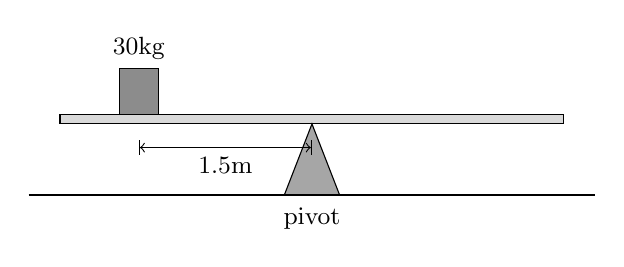
\begin{tikzpicture}
    \draw[fill=black!15] (-3.2,0.9) rectangle (3.2,1.02);
    \draw[fill=black!35] (-0.35,0) -- (0.35,0) -- (0,0.9) -- cycle; \draw[line width=0.6pt] (-3.6,0) -- (3.6,0);
    \draw[fill=black!45] (-2.45,1.02) rectangle (-1.95,1.6); \node[above, font=\small] at (-2.2,1.6) {\qty{30}{kg}};
    \draw[|<->|, line width=0.4pt] (-2.2,0.6) -- (0,0.6) node[midway, below, font=\small] {\qty{1.5}{m}};
    \node[font=\small] at (0,-0.3) {pivot};
  \end{tikzpicture}
\end{center}
\qpartL{a}{1}{Calculate the torque about the pivot due to the weight of the child.}{3}
\qpartL{b}{2}{A \qty{45}{kg} child sits on the other side. How far from the pivot must this child sit
for the seesaw to balance?}{4}
\qpartL{c}{2}{The \qty{45}{kg} child then moves further from the pivot. Explain why the seesaw starts
to rotate.}{4}
\end{saq}

% ---- Q10 (spin dryer)
\Needspace{24\baselineskip}
\begin{saq}{4}
The drum of a washing machine has a radius of \qty{0.25}{m}. During the spin cycle it rotates at
1200 revolutions per minute.
\qpartL{a}{1}{Calculate the angular velocity of the drum in \si{rad.s^{-1}}.}{3}
\qpartL{b}{2}{Calculate the centripetal acceleration of clothes pressed against the wall of the
drum.}{4}
\qpartL{c}{1}{The wall of the drum has small holes. Explain how the spin cycle removes water from
the clothes.}{2}
\end{saq}

% ---- Q11 (mass on a string: tension and breaking)
\Needspace{24\baselineskip}
\begin{saq}{6}
A \qty{0.50}{kg} mass on a string moves in a horizontal circle of radius \qty{0.80}{m} on a
frictionless table. It completes one revolution every \qty{0.40}{s}.
\qpartL{a}{1}{Calculate the speed of the mass.}{2}
\qpartL{b}{2}{Calculate the tension in the string.}{4}
\qpartL{c}{2}{The string breaks if the tension is more than \qty{150}{N}. Calculate the shortest
period of revolution the mass can have without the string breaking.}{5}
\qpartL{d}{1}{The radius is doubled, but the period stays at \qty{0.40}{s}. State how the tension
changes, with a reason.}{2}
\end{saq}

% ---- Q12 (practical investigation: force against 1/r)
% Data: v = 3.0 m/s kept constant, m = 0.050 kg; F = m v^2 / r; best-fit gradient 0.45 N m.
\Needspace{40\baselineskip}
\begin{saq}{6}
A student investigates how the centripetal force $F$ on a \qty{0.050}{kg} object depends on the
radius $r$ of its circular path. The speed of the object is kept constant at \qty{3.0}{m.s^{-1}}.
\begin{center}
  \renewcommand\arraystretch{1.5}
  \begin{tabular}{|l|*{5}{>{\centering\arraybackslash}p{14mm}|}}
    \hline
    \textbf{Radius $r$ (\si{m})} & 0.40 & 0.50 & 0.60 & 0.80 & 1.00\\ \hline
    \textbf{$\dfrac{1}{r}$ (\si{m^{-1}})} & & & & & \\[8pt] \hline
    \textbf{Force $F$ (\si{N})} & 1.14 & 0.89 & 0.76 & 0.55 & 0.46\\ \hline
  \end{tabular}
\end{center}
\qpartL{a}{1}{Complete the table by calculating $\dfrac{1}{r}$ for each radius.}{0}
\qpart{b}{3}{On the grid below, plot $F$ against $\dfrac{1}{r}$ and draw a line of best fit.}
\begin{center}
  \begin{tikzpicture}
    \begin{axis}[width=120mm, height=85mm, axis lines=left, xmin=0, xmax=3.0, ymin=0, ymax=1.4,
        xtick={0,0.5,...,3.0}, ytick={0,0.2,...,1.4}, minor x tick num=4, minor y tick num=3,
        grid=both, major grid style={black!45, line width=0.35pt}, minor grid style={black!18, line width=0.25pt},
        tick label style={font=\small}, label style={font=\small},
        xticklabel style={/pgf/number format/fixed, /pgf/number format/fixed zerofill, /pgf/number format/precision=1},
        yticklabel style={/pgf/number format/fixed, /pgf/number format/fixed zerofill, /pgf/number format/precision=1},
        xlabel={$\frac{1}{r}$ (\si{m^{-1}})}, ylabel={Force $F$ (\si{N})},
        scaled ticks=false, enlargelimits=false]
      \addplot[draw=none] coordinates {(0,0)};
    \end{axis}
  \end{tikzpicture}
\end{center}
\qpartL{c}{2}{Use the gradient of your line to determine the mass of the object, and compare it with
the known value.}{5}
\end{saq}

% ---- Q13 (compare circular and projectile motion)
\Needspace{110mm}
\begin{saq}{4}
Compare the velocity, acceleration and net force of an object in uniform circular motion with those
of a projectile.
\alines{10}
\end{saq}

% =====================================================================
\topictitle{Topic 3 - Motion in Gravitational Fields}

% ---- Q14 (Earth and Moon)
\begin{saq}{4}
The Moon has a mass of \qty{7.35e22}{kg} and orbits Earth at an average distance of
\qty{3.84e8}{m} (centre to centre).
\qpartL{a}{2}{Calculate the gravitational force between Earth and the Moon.}{5}
\qpartL{b}{2}{Calculate the orbital period of the Moon, in days.}{5}
\end{saq}

% ---- Q15 (g against distance)
\Needspace{36\baselineskip}
\begin{saq}{4}
\qpartL{a}{2}{Calculate the altitude above Earth's surface at which the gravitational field strength
is \qty{4.9}{N.kg^{-1}}.}{5}
\qpart{b}{2}{On the axes below, sketch a graph of the gravitational field strength $g$ against the
distance $r$ from the centre of Earth, from $r = r_\mathrm{E}$ to $r = 4r_\mathrm{E}$. Show the values
of $g$ at $r_\mathrm{E}$, $2r_\mathrm{E}$ and $4r_\mathrm{E}$.}
\begin{center}
  \begin{tikzpicture}
    \draw[axisline] (0,0) -- (8.2,0) node[right] {$r$};
    \draw[axisline] (0,0) -- (0,5.6) node[above] {$g$ (\si{N.kg^{-1}})};
    \foreach \k/\l in {1/r_\mathrm{E}, 2/2r_\mathrm{E}, 3/3r_\mathrm{E}, 4/4r_\mathrm{E}}
      {\draw (\k*1.9,0.08) -- (\k*1.9,-0.08) node[below, font=\small] {$\l$};}
    \foreach \y/\l in {1/2, 2/4, 3/6, 4/8, 5/10}
      {\draw (0.08,\y*1.0) -- (-0.08,\y*1.0) node[left, font=\small] {\l};}
  \end{tikzpicture}
\end{center}
\end{saq}

% ---- Q16 (Kepler's third law: moons of Jupiter)
\Needspace{30\baselineskip}
\begin{saq}{5}
The table shows data for four moons of Jupiter.
\begin{center}
  \renewcommand\arraystretch{1.5}
  \begin{tabular}{|l|c|c|}
    \hline
    \textbf{Moon} & \textbf{Orbital radius $r$ (\si{m})} & \textbf{Period $T$ (\si{s})}\\ \hline
    Io & \num{4.22e8} & \num{1.53e5}\\ \hline
    Europa & \num{6.71e8} & \num{3.07e5}\\ \hline
    Ganymede & \num{1.07e9} & \num{6.18e5}\\ \hline
    Callisto & \num{1.88e9} & \num{1.44e6}\\ \hline
  \end{tabular}
\end{center}
\qpartL{a}{2}{Show that these data are consistent with Kepler's third law.}{5}
\qpartL{b}{2}{Use the data to determine the mass of Jupiter.}{5}
\qpartL{c}{1}{The four moons have very different masses. Explain why this does not affect your
answer to part (a).}{2}
\end{saq}

% ---- Q17 (satellite at 600 km: speed and energy)
\Needspace{24\baselineskip}
\begin{saq}{5}
A \qty{1200}{kg} satellite is in a circular orbit at an altitude of \qty{600}{km}.
\qpartL{a}{2}{Calculate the orbital speed of the satellite.}{5}
\qpartL{b}{2}{Calculate the total energy of the satellite.}{5}
\qpartL{c}{1}{Explain why the total energy of the satellite is negative.}{2}
\end{saq}

% ---- Q18 (Kepler's second law: speeds at perihelion and aphelion)
\Needspace{34\baselineskip}
\begin{saq}{4}
A planet moves in an elliptical orbit around a star. At its closest point (perihelion) it is
\qty{1.0e11}{m} from the star and moves at \qty{30}{km.s^{-1}}. At its furthest point (aphelion) it is
\qty{1.5e11}{m} from the star.
\begin{center}
  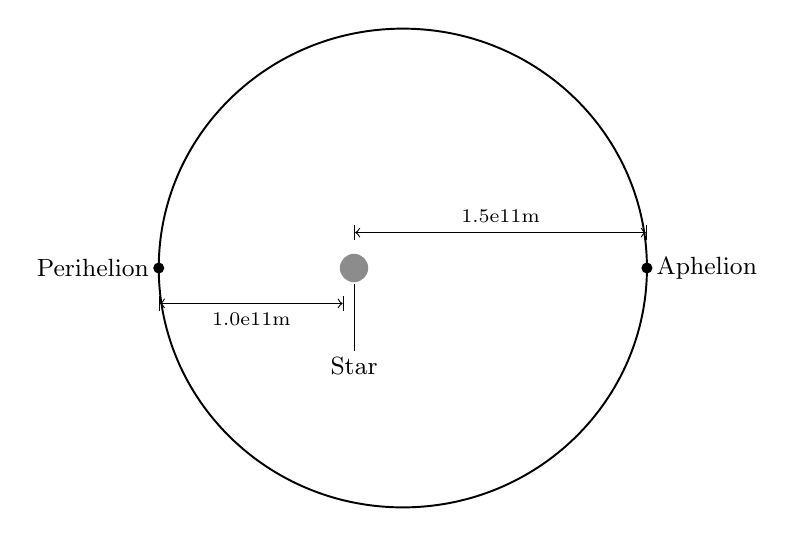
\begin{tikzpicture}
    \draw[line width=0.7pt] (0,0) ellipse (3.1 and 3.04);
    \fill[black!45] (-0.62,0) circle (0.18); \node[font=\small] at (-0.62,-1.25) {Star};
    \draw[line width=0.3pt] (-0.62,-0.2) -- (-0.62,-1.05);
    \fill (-3.1,0) circle (2pt) node[left, font=\small] {Perihelion};
    \fill (3.1,0) circle (2pt) node[right, font=\small] {Aphelion};
    \draw[|<->|, line width=0.4pt] (-3.1,-0.45) -- (-0.75,-0.45) node[midway, below, font=\scriptsize] {\qty{1.0e11}{m}};
    \draw[|<->|, line width=0.4pt] (-0.62,0.45) -- (3.1,0.45) node[midway, above, font=\scriptsize] {\qty{1.5e11}{m}};
  \end{tikzpicture}
\end{center}
\qpartL{a}{2}{Kepler's second law means that, at perihelion and aphelion, the product $rv$ is the
same. Calculate the speed of the planet at aphelion.}{4}
\qpartL{b}{2}{Explain, in terms of energy, why the planet's speed changes as it moves from
perihelion to aphelion.}{4}
\end{saq}

% ---- Q19 (escape velocity)
\Needspace{24\baselineskip}
\begin{saq}{4}
\qpartL{a}{1}{Calculate the escape velocity from Earth's surface.}{3}
\qpartL{b}{2}{Explain why the escape velocity does not depend on the mass of the rocket. Ignore air
resistance.}{4}
\qpartL{c}{1}{A satellite in low Earth orbit moves at about \qty{7.8}{km.s^{-1}}, which is less than
the escape velocity. Explain why it does not need to reach the escape velocity.}{2}
\end{saq}

% ---- Q20 (orbit with the same period as Mars' rotation)
\Needspace{30\baselineskip}
\begin{saq}{6}
A space agency wants to place a communications satellite in orbit around Mars, so that it always
stays above the same point on the surface of Mars. Mars has a mass of \qty{6.42e23}{kg}, a radius of
\qty{3.39e6}{m}, and rotates once every 24.6 hours.
\qpartL{a}{3}{Calculate the orbital radius needed for this satellite.}{7}
\qpartL{b}{1}{Calculate the altitude of this orbit above the surface of Mars.}{2}
\qpartL{c}{2}{Explain why this satellite must orbit above the equator of Mars, in the same direction
as Mars rotates.}{4}
\end{saq}

\end{document}
